\begin{figure}[H]
	\centering
	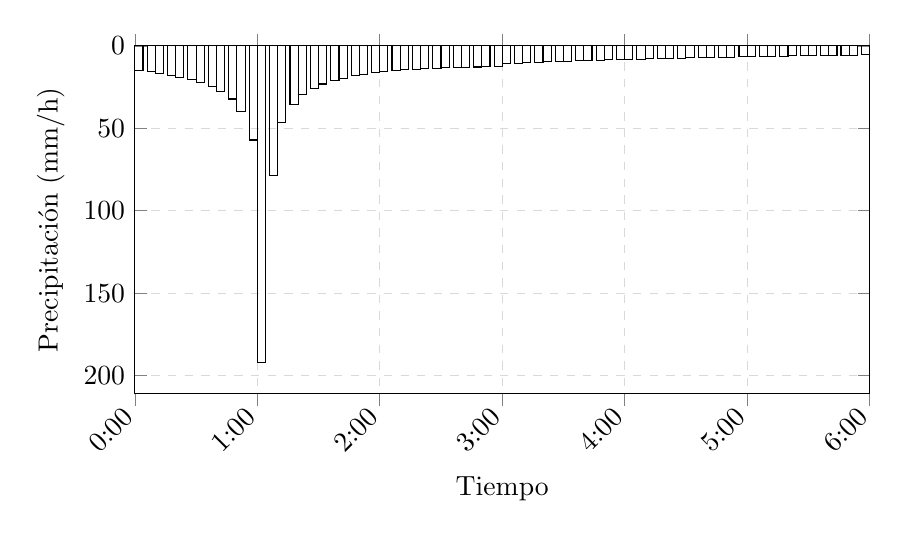
\begin{tikzpicture}
		\begin{axis}[
			width=0.9\textwidth,
			height=6cm,
			xlabel={Tiempo},
			ylabel={Precipitación (mm/h)},
			y dir=reverse,
			ymin=0,
			ymax=211,
			xmin=0,
			xmax=360,
			ybar,
			bar width=4,
			xtick={0, 60, 120, 180, 240, 300, 360},
			xticklabels={0:00, 1:00, 2:00, 3:00, 4:00, 5:00, 6:00},
			xticklabel style={rotate=45, anchor=east},
			grid=major,
			grid style={dashed, gray!30},
			]
			\addplot [
			draw=black,
			fill=none
			]
			coordinates {
				(2, 15.00) (8, 15.84) (12, 16.68) (18, 17.76) (22, 18.96)
				(28, 20.40) (32, 22.20) (38, 24.60) (42, 27.72) (48, 32.28)
				(52, 40.08) (58, 57.12) (62, 192.00) (68, 78.72) (72, 46.56)
				(78, 35.64) (82, 29.76) (88, 25.92) (92, 23.16) (98, 21.24)
				(102, 19.56) (108, 18.24) (112, 17.16) (118, 16.32) (122, 15.48)
				(128, 14.76) (132, 14.52) (138, 14.16) (142, 13.80) (148, 13.56)
				(152, 13.32) (158, 13.08) (162, 12.96) (168, 12.84) (172, 12.60)
				(178, 12.48) (182, 10.92) (188, 10.56) (192, 10.32) (198, 10.08)
				(202, 9.72) (208, 9.60) (212, 9.36) (218, 9.12) (222, 8.88)
				(228, 8.76) (232, 8.52) (238, 8.40) (242, 8.16) (248, 8.04)
				(252, 7.80) (258, 7.68) (262, 7.56) (268, 7.44) (272, 7.20)
				(278, 7.20) (282, 6.96) (288, 6.84) (292, 6.84) (298, 6.60)
				(302, 6.60) (308, 6.36) (312, 6.36) (318, 6.24) (322, 6.12)
				(328, 6.00) (332, 5.88) (338, 5.88) (342, 5.76) (348, 5.64)
				(352, 5.64) (358, 5.52)
			};
		\end{axis}
	\end{tikzpicture}
	\caption{Hietograma - GZ $T_r$=10 años (P=105.9 mm)}
	\label{fig:hyeto_kirpich_gz_Tr10_X100}
\end{figure}
